\chapter{Técnicas de Puño}

El capítulo dedicado a las ``Técnicas de Puños'' es un componente fundamental en el entrenamiento de Hwarangdo\textregistered. En esta sección, los practicantes exploran el arte y la precisión de los golpes, desarrollando habilidades esenciales para la defensa personal y el combate. Desde los conceptos básicos de la postura y el equilibrio hasta la aplicación efectiva de golpes, este capítulo proporciona una base sólida para la comprensión de cómo canalizar la fuerza y la energía a través de los puños. Los estudiantes aprenderán la importancia de la técnica y la velocidad, así como la coordinación y la sincronización necesarias para ejecutar golpes poderosos y precisos. A medida que avancen en este capítulo, ganarán una apreciación más profunda de la importancia de la disciplina y la perseverancia en el camino hacia la maestría en Hwarangdo\textregistered.

\section{Empuñadura de la Mano}

\subsection{Empuñadura Cerrada}

La empuñadura cerrada es un estilo común en muchas disciplinas marciales. En esta técnica, los dedos se cierran firmemente alrededor del puño, con el pulgar cubriendo los nudillos. Esto proporciona un sólido punto de impacto y permite realizar golpes potentes y precisos.

\begin{figure}[h]
	\centering
	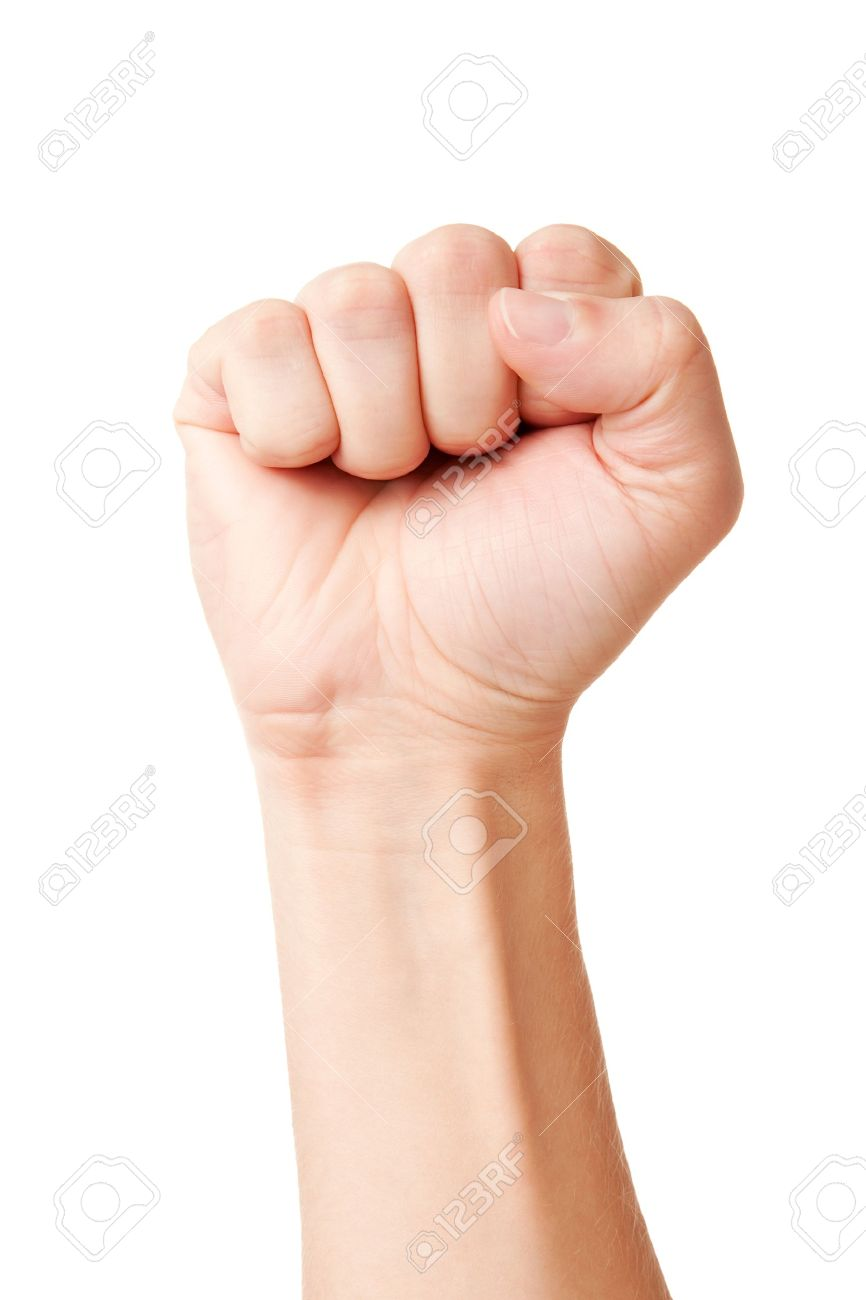
\includegraphics[width=0.2\linewidth]{images/Técnicas/puno_cerrado.jpg}
	\caption{Empuñadura Cerrada}
\end{figure}

\subsection{Empuñadura Abierta}

La empuñadura abierta es más relajada en comparación con la empuñadura cerrada. Los dedos están extendidos y relajados, con el pulgar ligeramente doblado hacia adentro. Esta técnica se utiliza en situaciones donde se necesita más control y precisión, como en las técnicas de bloqueo y control.

\begin{figure}[h]
	\centering
	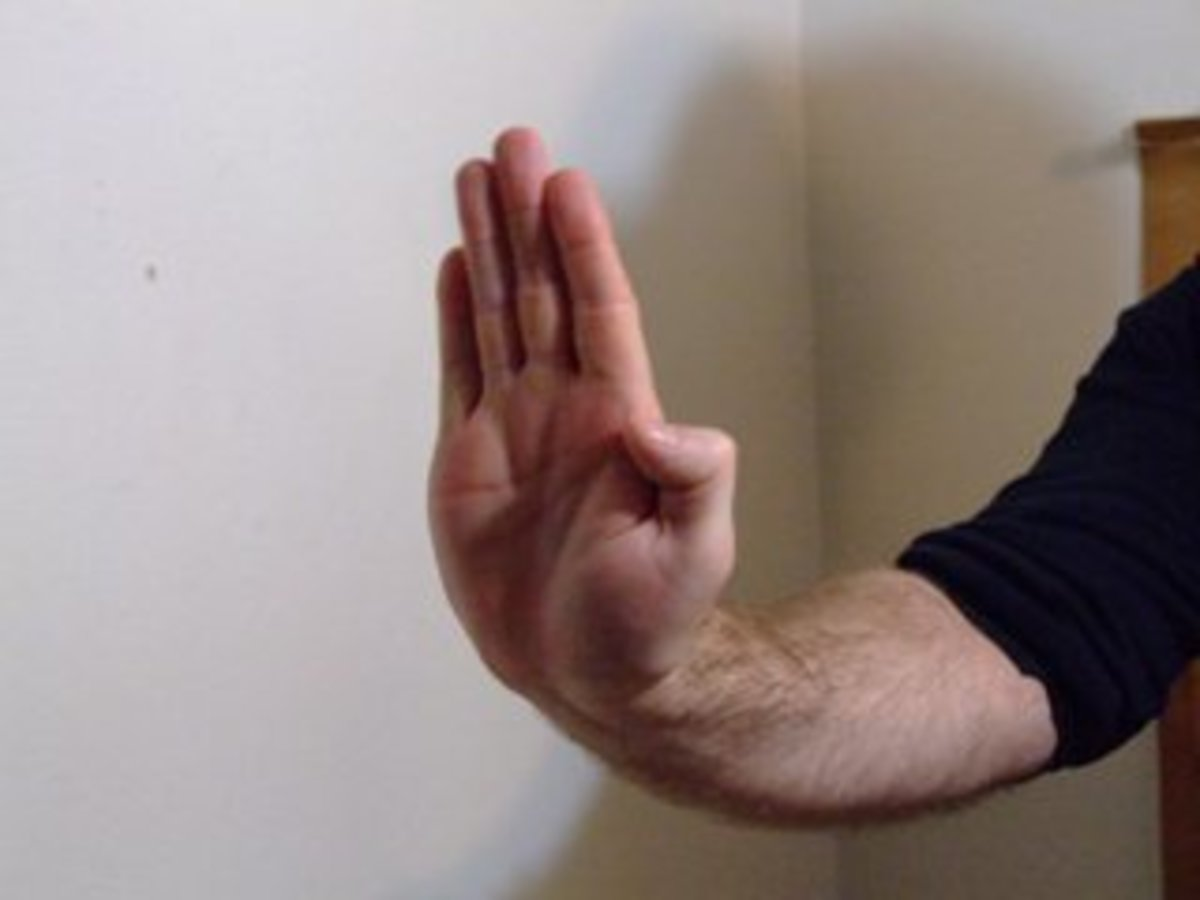
\includegraphics[width=0.2\linewidth]{images/Técnicas/puno_abierto.jpg}
	\caption{Empuñadura Abierta}
\end{figure}

